\author{Thomas Backman, exscape@gmail.com}
\date{\today}
\title{6.002x notes}

% Use a nice font
\documentclass[12pt,a4paper]{report}

% Custom package!
% For strikethrough.
\usepackage{cancel}

% Create clickable URLs
%\usepackage{url}

% Multiline comments
\usepackage{verbatim}

\usepackage{graphicx}

%\usepackage{pgfplots}

% Aligned equations and more
\usepackage{amsmath}
\usepackage{mathtools}

% Links in the table of contents
\usepackage[colorlinks=true, urlcolor=blue,linkcolor=red]{hyperref}

% Fix margins and indentation
\usepackage[cm]{fullpage}
\addtolength{\oddsidemargin}{-0.75cm}
\addtolength{\evensidemargin}{-0.75cm}
\addtolength{\topmargin}{-0.5cm}
\setlength{\parindent}{0in}

% For circuit diagrams
\usepackage{siunitx}
\usepackage[american,siunitx]{circuitikz}

\begin{document}

\maketitle

\tableofcontents

%%%%%%%%%%%%%%%%%%%%%%%%
%% Formulas and such %%%
%%%%%%%%%%%%%%%%%%%%%%%%

\chapter{Formulas and such}

\section{Intro}

This chapter contains several common formulas etc., without any further explanation of how they are derived.

\section{Components in series and parallel}

Series resistances add:

\[ R_s = R_1 + R_2 + R_3 + \cdots \]

Parallel resistances diminish:

\[ R_p = \frac{1}{ \frac{1}{R_1} + \frac{1}{R_2} + \frac{1}{R_3} + \cdots} \]

Impedances behave like resistances.\\

Series capacitances diminish:

\[ C_s = \frac{1}{ \frac{1}{C_1} + \frac{1}{C_2} + \frac{1}{C_3} + \cdots} \]

Parallel capacitances add:

\[ C_p = C_1 + C_2 + C_3 + \cdots \]

Series inductances add:

\[ L_s = L_1 + L_2 + L_3 + \cdots \]

Parallel inductances diminish:

\[ L_p = \frac{1}{ \frac{1}{L_1} + \frac{1}{L_2} + \frac{1}{L_3} + \cdots} \]

For the special case of two components of the diminshing type (x being a dummy variable):

\[ \frac{1}{ \frac{1}{x_1} + \frac{1}{x_2} } = \frac{x_1 \cdot x_2}{x_1 + x_2} \]

\section{Digital}

\subsection{Noise margins}
\begin{align*}
  NM_H &= V_{OH} - V_{IH}\\
  NM_L &= V_{IL} - V_{OL}\\
\text{Forbidden region} &= V_{IH} - V_{IL}
\end{align*}

\section{MOSFETs}

\subsection{SCS model}
\[ 
 i_{DS} = \begin{cases}
   \frac{K}{2}(v_{GS} - V_T)^2 & \text{for $v_{GS} \ge V_T, v_{DS} \ge v_{GS} - V_T$} \\
   0 & \text{for $v_{GS} < V_T$}
 \end{cases}
\]
The above covers saturation and cutoff regions only (the SCS model).

\subsection{SR model}

\[ 
  i_{DS} = \begin{cases}
  \frac{V_{DS}}{R_{ON}} & \text{for $V_{GS} \ge V_T$} \\
  0 & \text{otherwise}
  \end{cases}
\]

Alternatively:
\[ 
  R_{DS} = \begin{cases}
  R_{ON} & \text{for $V_{GS} \ge V_T$} \\
  \infty & \text{otherwise}
  \end{cases}
\]

Used for digital circuits only (in this course).

\section{State devices / energy storage devices}
This section assumes time-invariant devices, i.e. capacitance/inductance is a fixed value, and not a function of time.

\subsection{Capacitors}

The current through a capacitor is a function of the \emph{rate of change} of voltage:

\[ i(t) = C \frac{dv(t)}{dt} \]

To find the voltage over a capacitor, we need to know its full history:

\[ v(t) = \frac{1}{C} \int_{-\infty}^{t} i(t) dt \]

... or we can simply do it by knowing the current through it between $t_1$ and $t_2$, plus the initial voltage:

\[ v(t_2) = \frac{1}{C} \int_{t_1}^{t_2} i(t) dt + v(t_1) \]

The energy stored in a capacitor is:

\[ E = \frac{1}{2} C v^2 \]

\subsection{Inductors}

The voltage over an inductor is a function of the \emph{rate of change} of current:

\[ v(t) = L \frac{di(t)}{dt} \]

To find the current through a capacitor, we need to know its full history:

\[ i(t) = \frac{1}{L} \int_{-\infty}^t v(t) dt \]

... or we can simply do it by knowing the voltage over it between $t_1$ and $t_2$, plus the initial current through it:

\[ i(t_2) = \frac{1}{L} \int_{t_1}^{t_2} v(t) dt + i(t_1) \]

The energy stored in an inductor is:

\[ E = \frac{1}{2} L i^2 \]

\newpage

\section{Second order circuits, impedance, filters}

Canonical form of the characteristic equation for second-order circuits; use this to match up the values of $\alpha$ and $\omega_0$ for a circuit:

\[ s^2 + 2\alpha s + {\omega_0}^2 = 0 \]

\subsection{For all LC and RLC circuits:}

\[ \text{Natural/undamped resonant radian frequency: } \omega_0 \text{ (rad/s)} \]
\[ \text{Damping factor: } \alpha \text{ (rad/s)} \]

Note that zeta ($\zeta$) is used as a damping factor in many texts; it is defined as
\[ \zeta = \frac{\alpha}{\omega_0} \text{ (dimensionless)} \]

The bandwidth $\Delta \omega$, i.e. the \emph{width} of the frequency \emph{band} that is above $\displaystyle \frac{1}{\sqrt{2}}$ times the input amplitude, is given by

\[ \Delta \omega = 2 \alpha \text{ (rad/s) (measured at } \frac{1}{\sqrt{2}} \text{ points)} \]

\[ \text{Quality factor: } Q = \frac{\omega_0}{2\alpha} \text{ (dimensionless)} \]

RLC circuits can be underdamped, overdamped, or critically damped.

\[ \text{Underdamped: } \omega_0 > \alpha \text{ or, equivalently, } Q > \frac{1}{2} \text { or, equivalently, } \zeta < 1 \]
\[ \text{Overdamped: } \omega_0 < \alpha \text{ or, equivalently, } Q < \frac{1}{2} \text { or, equivalently, } \zeta > 1 \]
\[ \text{Critically damped: } \omega_0 = \alpha \text{ or, equivalently, } Q = \frac{1}{2} \text { or, equivalently, } \zeta = 1 \]

When they are \emph{underdamped}, the \emph{damped resonant frequency} $\omega_d$ is given by
\[ \omega_d = \sqrt{{\omega_0}^2 - \alpha^2} \]
The naming here might be confusing; the \emph{damped} frequency is used for \emph{underdamped} systems. The reason is that the \emph{undamped} frequency is used for systems with no damping whatsoever, i.e. LC circuits with no resistor.\\
Underdamped RLC circuits are the only kind that oscillate, so the natural frequency is less interesting for overdamped circuits.

\subsection{Series RLC circuits}

\[ \omega_0 = \frac{1}{\sqrt{LC}} \text{ rad/s} \]
\[ f_0 = \frac{1}{2\pi \sqrt{LC}} \text { Hz} \]
\[ \alpha = \frac{R}{2L} \text{ rad/s} \]
\[ \Delta \omega = 2\alpha = \frac{R}{L} \text { rad/s} \]
\[ \text{Period: } \frac{2\pi}{\omega_0} = 2\pi \sqrt{LC} \text { seconds} \]
\[ Q = \frac{\omega_0}{2\alpha} = \frac{L}{R\sqrt{LC}} \text { (dimensionless)} \]

\subsection{Parallel RLC circuits}

\[ \omega_0 = \frac{1}{\sqrt{LC}} \text{ rad/s} \]
\[ f_0 = \frac{1}{2\pi \sqrt{LC}} \text { Hz} \]
\[ \alpha = \frac{1}{2RC} \text{ rad/s} \]
\[ \Delta \omega = 2\alpha = \frac{1}{RC} \text { rad/s} \]
\[ \text{Period: } \frac{2\pi}{\omega_0} = 2\pi \sqrt{LC} \text { seconds} \]
\[ Q = \frac{\omega_0}{2\alpha} = \frac{RC}{\sqrt{LC}} \text { (dimensionless)} \]

\subsection{Frequency- to time-domain conversion}
You can find the time-domain behavior of a circuit to sinusoidal input from nothing but a complex amplitude of the form $V_x$:
\[ v_X(t) = |V_x| \cos{(\omega t + \angle V_x)} \]
See below for information about how to calculate the magnitude $|z|$ and the angle $\angle z$ of a complex number.

\subsection{Complex algebra}
A few properties of complex numbers that are necessary to know:

\[ |a + jb| = \sqrt{a^2 + b^2} \]
\[ \angle (a + jb) = \arctan{(\frac{b}{a})} \text{ or, preferably, } \text{atan2}(a, b) \]

\[ |a + j0| = a \text { if $a > 0$; otherwise, the magnitude is just the absolute value } |a| \]
\[ |0 + jb| = b \]
\[ |0 - jb| = b \]

\[ \angle (a + j0) = 0 \]
\[ \angle (0 + jb) = \frac{\pi}{2} \]
\[ \angle (0 - jb) = -\frac{\pi}{2} \]

\[ |z_1 \cdot z_2| = |z_1| \cdot |z_2| \]
\[ \left| \frac{z_1}{z_2} \right| = \frac{|z_1|}{|z_2|} \]

\[ \angle (z_1 \cdot z_2) = \angle z_1 + \angle z_2 \]
\[ \angle \left( \frac{z_1}{z_2} \right) = \angle z_1 - \angle z_2 \]

When finding angles, it's best to use a function which is capable of giving correct answers in all quadrants of the unit circle. The ``atan2'' function was created in many computer languages for this purpose. It is equal to $\displaystyle \arctan{(\frac{b}{a})}$ for some inputs, but not all; arctan() cannot differentiate between all quadrants, because $\displaystyle \arctan{\left( \frac{-a}{-b}\right )} = \arctan{\left( \frac{a}{b}\right) }$ and likewise, $\displaystyle \arctan{\left( \frac{-a}{b}\right )} = \arctan{\left( \frac{a}{-b}\right) }$. Thus, the atan2 function has two arguments, and when using it, the angle of a complex number $a + jb$ is simply $\text{atan2}(a, b)$.\\
The angle of a fully real number is always $0$, and the angle of a fully imaginary number always either $\displaystyle \frac{\pi}{2}$ (for positive imaginary numbers) or $\displaystyle -\frac{\pi}{2}$ (for negative imaginary numbers).

One definition of atan2, if you are not using math software that has it, is:

\[ \text{atan2}(b, a) = 2\arctan{(\frac{b}{\sqrt{a^2 + b^2} + a})} \]

However, note that these notes use an atan2 function that is defined with the variables in the opposite order, i.e. atan2(a, b); specifically, Mathematica's ArcTan[a, b] function.


\subsection{Impedances}

\[ \text{Resistor: } Z_R = R \]
\[ \text{Capacitor: } Z_C = \frac{1}{j\omega C} \]
\[ \text{Inductor: } Z_L = j\omega L \]

%%%%%%%%%%%%%%%%%%%%%%%%
%%% Circuit analysis %%%
%%%%%%%%%%%%%%%%%%%%%%%%

\chapter{Circuit analysis}

\section{Thevenin equivalent circuits}

Say we have an capacitor circuit to analyze:

\begin{circuitikz}[scale=1.2]
\draw (0,0) node [ground] {} to [V=$V_S$] (0,3)
                             to [R=$R_1$]  (3,3)
                             to [R=$R_2$]  (6,3)
                             to [C=$C$, v=$v_C$]   (6,0);

\draw (3,3)                  to [R=$R_3$]  (3,0);
\draw (0,0)                  to           (6,0);
\end{circuitikz}
\\

Since this is a linear network, we can simplify it by calculating its \emph{Thevenin equivalent}. Consider the network as seen from the port where the capacitor is attached:

\begin{circuitikz}[scale=1.2]
\draw (0,0) node [ground] {} to [V=$V_S$] (0,3)
                             to [R=$R_1$]  (3,3)
                             to [R=$R_2$, -o]  (6,3);

\draw (3,3)                  to [R=$R_3$]  (3,0);
\draw (0,0)                  to [short, -o]         (6,0);
\draw (6,0)                  to [open, v>=$V_{TH}$] (6,3);
\end{circuitikz}
\\

$V_{TH}$, the open circuit voltage, will be given by the voltage divider formed by $R_3$ and $R_1$:

\[ V_{TH} = \frac{R_3}{R_1 + R_3} \cdot V_S \]

Since no current flows at the port (for the \emph{open circuit} voltage!), $R_2$ doesn't contribute at all.

We also want to measure the resistance ``looking in'' to this port; this will be the Thevenin resistance $R_{TH}$. To do this, we turn off all \emph{independant} voltage and current sources, by replacing all current sources with \emph{opens} and all voltage sources with \emph{short circuits}.\\
Leave dependant sources in the circuit!

\begin{circuitikz}[scale=1.2]
\draw (0,0)                  to [short] (0,3)
                             to [R=$R_1$]  (3,3)
                             to [R=$R_2$, -o]  (6,3);

\draw (3,3)                  to [R=$R_3$]  (3,0);
\draw (0,0)                  to [short, -o]         (6,0);
\draw (6,0)                  to [open] (6,3);
\end{circuitikz}

\[ R_{TH} = R_2 + (R_1 || R_3) = R_2 + \frac{R_1 \cdot R_3}{R_1 + R_3} \]

Now that we know the Thevenin voltage $V_{TH}$ and the Thevenin resistance $R_{TH}$, we can replace the circuit with a voltage source of voltage $V_{TH}$ volts in series with a resistor of value $R_{TH}$ ohm, and place the capacitor back into the circuit:

\begin{circuitikz}[scale=1.2]
\draw (0,0) node [ground] {} to [V=$V_{TH}$] (0,3)
                             to [R=$R_{TH}$] (3,3)
                             to [C=$C$, v=$v_C$]      (3,0);
\draw (0,0)                  to              (3,0);
\end{circuitikz}
                             
Our previous circuit has now turned into a simple RC circuit, which is easier to analyze. See the chapter on RC circuits.\\

As a side note, another way of measuring the Thevenin resistance is to short circuit the output node, calculate/measure the short-circuit current (with all sources left intact, of course), and calculate $R_{TH}$ as $\frac{V_{TH}}{I_{SC}}$.\\

In summary:

$\bullet$ Calculate/measure the open circuit voltage $V_{TH}$ at the port\\
$\bullet$ Turn off all independent sources (make short circuits of voltage sources, and open circuits of current sources), but leave dependant sources intact\\
$\bullet$ Calculate/measure the resistance $R_{TH}$ at the port terminal pair\\
$\bullet$ Replace the original circuit with a series circuit of a voltage source (voltage $V_{TH}$ volts), a resistor (resistance $R_{TH}$ ohm) and the element you want to analyze.

\newpage

\section{Norton equivalent circuits}
Nortan equivalent circuits are very similar to Thevenin equivalents, but use a \emph{current source} in \emph{parallel} with a resistor rather than a \emph{voltage source} in \emph{series} with a resistor.

To convert a circuit to its Norton equivalent:

$\bullet$ Calcurate/measure the \emph{short circuit current}, i.e. the current that would flow through the output port if we were to short-circuit it. The result is the Norton current $I_N$.\\
$\bullet$ Turn off all independent sources (make short circuits of voltage sources, and open circuits of current sources), but leave dependant sources intact.\\
$\bullet$ Calculate/measure the resistance at the port terminal pair; the result is the Norton resistance $R_N$.\\
$\bullet$ Replace the original circuit with a parallel circuit of a current source (current $I_N$ amperes), a resistor (resistance $R_N$ ohm) and the element you want to analyze.\\

\begin{circuitikz}[scale=1.2]
\draw (0,0) node [ground] {} to [I=$I_N$] (0,3);
\draw (0,3) to (3,3);
\draw (3,3) to [R=$R_N$] (3,0);
\draw (6,3) to [C=$C$, v=$v_C$] (6,0);
\draw (6,0) to (0,0);
\draw (6,3) to (3,3);
\end{circuitikz}
\\

Note that since the method for calculating the equivalent resistance is identical for the Thevenin and Norton methods, $R_N = R_{TH}$.
It is easy to convert between one and the other:

\[ R_N = R_{TH} \]
\[ I_N = \frac{V_{TH}}{R_{TH}} \]
\[ V_{TH} = I_N \cdot R_N \]

%%%%%%%%%%%%%%%%%%%%%%%%%%%
%%% Small signal method %%%
%%%%%%%%%%%%%%%%%%%%%%%%%%%

\chapter{Small signal method}
\section{Deriving small signal models}

For a device with $i_D = f(v_D)$, the small signal current $i_d$ is given by

\[ \underbrace { \left. \frac{\partial f(v_D)}{\partial v_D} \right|_{v_D=V_D} }_{\displaystyle g_m} \cdot v_d \]

where $v_d$ is the small signal input voltage.\\
In other words, take the partial derivative of the V-I relation, with respect to the voltage. That gives $g_m$, the transconductance. The transconductance multiplied by the small signal input voltage $v_d$ gives the small signal current.\\

As an example, a MOSFET in the saturation region has $i_{DS} = f(v_{GS}) = \frac{K}{2}(v_{GS} - V_T)^2$:

\[ i_{ds} = \underbrace { \left. \frac{ \partial \frac{K}{2}(v_{GS} - V_T)^2 }{\partial v_{GS}} \right|_{v_{GS}=V_{GS} }}_{\displaystyle g_m} \cdot v_{gs} = \underbrace{ K(V_{GS} - V_T)}_{\displaystyle g_m} \cdot v_{gs} \]

Note the difference between $v_{GS}$ (the total gate-to-source voltage), $V_{GS}$ (the DC bias voltage) and $v_{gs}$ (the small signal / incremental voltage). \\
Also note that the value of $g_m$ depends not only on the MOSFET parameters $K$ and $V_T$, but also on the user-chosen DC bias voltage $V_{GS}$.\\

Here's a table of common circuit elements and their small signal equivalents:\\

\begin{tabular}{| l | l |}
\hline
Device & Small signal replacement \\ \hline
Resistor, R $\Omega$        & Resistor, R $\Omega$ \\ \hline
Voltage source, V volts     & Short circuit \\ \hline
Current source, I amps      & Open circuit \\ \hline
MOSFET in saturation region & VCCS, $i_{ds} = g_m v_{gs}$, $g_m = K(V_{GS} - V_T)$ \\ \hline 
MOSFET with gate/drain tied together & Resistor, $\displaystyle \frac{1}{K(V_{DS} - V_T)} \Omega$ (for $v_{DS} > V_T$) \\ \hline
\end{tabular}

\newpage

\section{Multivariable small signal models}
In some cases, it might be necessary to make a small signal model of a device where the current depends on more than one variable. An example (that will be used here) in 6.002x is the (probably hypothetical) ``NewFET'' in the week 6 homework.\\
In this case, we take the partial derivative of the gate-to-source voltage at the bias point times the small signal voltage $vgs$, \emph{plus} the partial derivative of the drain-to-source voltage at the bias point times the small signal voltage $vds$.

First, the properties of the NewFET:

\[ 
iDS = \begin{cases}
  0 & \text{for $v_{GS} < V_T$} \\
  K(v_{GS} - V_T) {v_{DS}}^2 & \text{for $v_{GS} \ge V_T$}
\end{cases}
\]
\\
The small signal model will look like this:

\begin{circuitikz}[scale=1.2]
\draw (3,2.5) to [cI=$g_m v_{gs}$, *-*] (3,0);
\draw (5,2.5) to [R=$r_o$, *-*] (5,0);
\draw (5,2.5) to [short, i<=$i_{ds}$] (6,2.5) node {\quad D};
\draw (5,0) to (6,0) [short] node {\quad S};
\draw (7,2.5) to [open, v=$v_{ds}$] (7,0);
\draw (3,2.5) to (5,2.5);
\draw (0,0) to (5,0);
\draw (-0.25,0) node {S} [open] to (0,0);
\draw (0,2.5) [open, v=$v_{gs}$, *-*] to (0,0);
\draw (-0.25,2.5) node {G} [open] to (0,2.5);

\end{circuitikz}
\\

The small signal current $i_{ds}$ will depend on both $v_{gs}$ and $v_{ds}$, in this manner:

\[ 
  i_{ds} = v_{gs} \underbrace{ \left. \frac{\partial i_D}{\partial v_{GS}} \right|_{v_{GS}=V_{GS}}}_{\displaystyle g_m} + v_{ds} \underbrace{ \left. \frac{\partial i_D}{\partial v_{DS}} \right|_{v_{DS}=V_{DS}}}_{\displaystyle 1/r_o}
\]

$g_m$ will be the regular transconductance, calculated the same as with MOSFETs (see the above section):

\[ 
  g_m = \left. \frac{\partial i_D}{\partial v_{GS}} \right|_{v_{GS}=V_{GS}} = \left. \frac{\partial K(v_{GS} - V_T) {v_{DS}}^2}{ \partial v_{GS}} \right|_{v_{GS}=V_{GS}} = K {V_{DS}}^2
\]

$r_o$ will be the \emph{reciprocal} of the partial of $i_D$ with respect to $v_{DS}$:\\
(In other words, the partial will give a conductance, and we want a resistance.)

\[ 
  \frac{1}{r_o} = \left. \frac{\partial i_D}{\partial v_{DS}} \right|_{v_{DS}=V_{DS}} = \left. \frac{\partial K(v_{GS} - V_T) {v_{DS}}^2}{ \partial v_{DS}} \right|_{v_{DS}=V_{DS}} = 2 K V_{DS} (V_{GS} - V_T)
\]
So
\[ r_o = \frac{1}{2 K V_{DS} (V_{GS} - V_T)} \]

From these equations and the circuit diagram, we see that 
\[
 i_{ds} = \frac{v_{ds}}{r_o} + g_m v_{gs} = v_{ds} \cdot 2 K V_{DS} (V_{GS} - V_T) + K {V_{DS}}^2 \cdot v_{gs} 
 \]

Note that, although the expression contains a square term (${V_{DS}}^2$), it is still linear, as the square term is a constant - the bias voltage $V_{DS}$ should not change, or the entire small signal model will be incorrect either way.

So, the result is not quite the simplest of expressions, but when the bias constants are replaced with their actual bias values, the result is of the form

\[ i_{ds} = C_{1} v_{ds} + C_{2} v_{gs} \]

where $C_1$ and $C_2$ are constants.

%%%%%%%%%%%%%%%%%%%%%%%%%%%%
%%% First-order circuits %%%
%%%%%%%%%%%%%%%%%%%%%%%%%%%%

\chapter{First-order circuits}
\section{Series RC circuits}

\begin{circuitikz}[scale=1.2]
\draw (0,0) node [ground] {} to [V=$V_S$] (0,3)
					  to [R=$R$]     (3,3)
					  to [C=$C$, v<=$v_C$]	(3,0);
\draw (3,0) to (0,0);
\end{circuitikz}
\\

We start off by writing down a KCL equation for the unknown node voltage $v_C$:\\
\[ \frac{v_C - V_S}{R} + C \frac{dv_C}{dt} = 0 \]

Rewrite the equation to get it in the form we prefer:

\[ RC \frac{dv_C}{dt} + v_C = V_S \]

To solve this first-order linear differential equation, we'll use the method of particular and homogeneous solutions, where we need to find two solutions to the differential equation: the first (the \emph{particular} solution) is \emph{any} solution that makes the equation true:

\[ RC \frac{dv_{Cp}}{dt} + v_{Cp} = V_S \]

We see here that if we pick $v_{Cp} = V_S$, where $V_S$ is a constant, thus making $\frac{dV_S}{dt} = 0$, this equation is indeed true; since the first term becomes 0, all that remains is $V_S = V_S$ - which is clearly true!\\
Thus, we've found the particular solution:

\[ v_{Cp} = V_S \]

The next step in this method is to find a solution to the homogeneous equation, where $V_S$ (the ``input drive'') is zero:

\[ RC \frac{dv_{Ch}}{dt} + v_{Ch} = 0 \]

We need a function such that its derivative is the function itself times a constant. $e^x$ comes to mind - more specifically, the solution will have some (still unknown) coefficients $A$ and $s$, such that:

\[ v_{Ch} = Ae^{st} \]

We substitute $Ae^{st}$ into the homogeneous equation and end up with:

\[ RC \frac{dAe^{st}}{dt} + Ae^{st} = 0 \]

We calculate the derivative and replace the $\frac{d}{dt}$ term with it:

\[ RCAs e^{st}  +Ae^{st} = 0 \]

Divide both sides by $Ae^{st}$:

\[ RCs + 1 = 0 \]
\[ RCs = -1 \]
\[ s = -\frac{1}{RC} \]

We've thus found one of our two constants.\\
The total solution to the differential equation will be the \emph{sum} of the particular and homogeneous solutions, so the next step is to add them together:

\[ v_C(t) = v_{Cp}(t) + v_{Ch}(t) \]
\[ v_C(t) = V_S + Ae^{-\frac{1}{RC} \cdot t} \]

All that remains to do is to find the value of the constant $A$. To do so, we substitute $v_C$ for the given initual condition $v_C(0) = V_0$, while setting $t = 0$:

\[ V_0 = V_S + Ae^0 \]
\[ V_0 = V_S + A \]
\[ A = V_0 - V_S \]

We've thus found the full solution:

\[ v_C(t) = V_S + (V_0 - V_S)e^{-\frac{t}{RC}} \]

\newpage

\section{Parallel RC circuit with a current source}

\begin{circuitikz}[scale=1.2]
\draw (0,0) node [ground] {} to [I=$I$] (0,3);
\draw (0,3) to (2,3);
\draw (2,3) to [R=$R$] (2,0);
\draw (2,3) to (4,3);
\draw (4,3) to [C=$C$, v=$v_C$] (4,0);
\draw (4,0) to (0,0);
\end{circuitikz}
\\

To save time (and space): the differential equation we end up with is exactly the same as for the series circuit above, with the sole difference that $IR$ replaces $V_S$, where $I$ is the current source drive current, and $R$ is the parallel resistor's resistance.\\
Since the resulting equation

\[ RC \frac{dv_C}{dt} + v_C = IR \]
is of the same form as the one for the series circuit, the solution is also the same:

\[ v_C(t) = IR + (V_0 - IR)e^{-\frac{t}{RC} } \]

%%%%%%%%%%%%%%%%%%%%%%%%%%%%%
%%% Second-order circuits %%%
%%%%%%%%%%%%%%%%%%%%%%%%%%%%%

\chapter{Second-order circuits}
\section{Series RLC circuits}

\begin{circuitikz}[scale=1.2]
\draw (0,0) node [ground] {} to [V=$V_S$] (0,3)
                     to [L=$L$, v<=$v_L$]     (2,3)
					  to [R=$R$, v<=$v_R$, i>=$i$]     (4,3)
					  to [C=$C$, v<=$v$]	(4,0);
\draw (4,0) to (0,0);
\end{circuitikz}

We know that the current $i$ relates to the capacitor voltage:

\[ i = C \frac{dv}{dt} \]

Since this is a series circuit, that current goes through all elements.

By KVL, we can add up the voltage drops around the loop, with the proper sign. I'll go clockwise, and start in the bottom left:

\[ -V_S + v_L + v_R + v = 0 \]

If we solve for $V_S$:

\[ V_S = v_L + v_R + v \]

Now, let's use the element laws for the inductor and resistor, and substitute them into the above:

\[ V_S = L \frac{di(t)}{dt} + R i(t) + v(t) \]
\newpage
We know that $i(t) = C \frac{dv}{dt}$, so let's substitute that back in. Let's also differentiate, in case of the inductor, to reduce the mess of nested differentiation operators:

\[ V_S = LC \frac{d^2v(t)}{dt^2} + RC \frac{dv}{dt} + v(t) \]

There we go; we now have a second-order, linear, constant coefficient ordinary differential equation.\footnote{I just love these overly verbose classifications.}\\

We'll use the same method to solve it as we did for the first-order ones, namely the method of particular and homogeneous solutions. First we first the particular solution (\emph{any} solution that makes the equation true), then the homogeneous solution (a solution to the equation with the input drive $V_S$ set to 0), and finally we add the two together to find the total solution.\\

As for the particular solution, just as in the first-order case, we try $v(t) = V_S$ and see that the two derivatives both go to zero (as $V_S$ is a constant), and so we end up with

\[ V_S = V_S \]

which tells us that $V_S$ indeed is a particular solution. On to the homogeneous one, i.e. the solution to 

\[ LC \frac{d^2v(t)}{dt^2} + RC \frac{dv}{dt} + v(t) = 0\]

Again, like in the first-order case, we try the form 

\[ v(t) = Ae^{st} \]

where $A$ and $s$ are constants we'll have to find later. So, we substitute $Ae^{st}$ for $v(t)$, and differentiate where necessary, which gives us

\[ LC As^2 e^{st} + RC As e^{st} + A e^{st} = 0 \]

We can cancel out a ton of the above, by dividing both sides by $A e^{st}$:

\[ LC \cancel{A} s^2 \cancel{e^{st}} + RC \cancel{A}s \cancel{e^{st}} + \cancel{A e^{st}} = 0 \]
What remains is

\[ LC s^2 + RC s + 1 = 0 \]

Divide by LC throughout:

\[ s^2 + \frac{R}{L} s + \frac{1}{LC} = 0 \]

We've thus arrived at the \emph{characteristic equation}, which describes most details of the circuit's behavior. There's a canonical form to write such an equation:

\[ s^2 + 2\alpha s + {\omega_0}^2 = 0 \]

So, in the case of the series RLC circuit, the values of $\alpha$ and $\omega_0$ would have to be

\[ \alpha = \frac{R}{2L} \]
and
\[ \omega_0 = \frac{1}{\sqrt{LC}} \]

$\alpha$ relates to the damping factor of the circuit (sometimes the damping factor, $\displaystyle \zeta = \frac{\alpha}{\omega_0}$, is used) - that is, the ringing second-order circuits can produce will decay faster for a larger value of $\alpha$. Meanwhile, $\omega_0$ is the \emph{undamped resonance frequency} of the circuit (in radians/second), the same as in undriven LC circuits. However, this might not be the frequency of interest in a RLC circuit - more on that later.\\

Let's get back to solving the differential equation. Remember, we only found the homogeneous solution - we still haven't figured out the values of $s$ or $A$.

The next step would be to find the roots of the characteristic equation:

\[ s^2 + 2\alpha s + {\omega_0}^2 + 0 \]

The quadratic formula will work nicely on this. The two roots are:

\[ s_1 = -\alpha + \sqrt{\alpha^2 - {\omega_0}^2} \]
\[ s_2 = -\alpha - \sqrt{\alpha^2 - {\omega_0}^2} \]

The full solution to the homogeneous solution will then be

\[ v_H = A_1 e^{s_1 t} + A_2 e^{s_2 t} \]

However, we've now found $s_1$ and $s_2$, so we can fill them in:
\large
\[ v_H = A_1 e^{(-\alpha + \sqrt{\alpha^2 - {\omega_0}^2}) t} + A_2 e^{(-\alpha - \sqrt{\alpha^2 - {\omega_0}^2}) t} \]
\normalsize

Then, the total solution (prior to finding $A_1$ and $A_2$, and also prior to simplifying) is:

\[ v(t) = V_S + A_1 e^{(-\alpha + \sqrt{\alpha^2 - {\omega_0}^2}) t} + A_2 e^{(-\alpha - \sqrt{\alpha^2 - {\omega_0}^2}) t} \]

After some magic\footnote{Sorry, but I don't quite follow the entire process myself yet. Since this part was cut out from the lectures in order to save time (after ~14 videos going through this process so far), I will do the same.} and making the definition $\omega_d = \sqrt{{\omega_0}^2 - \alpha^2}$, the total solution ends up looking like this, for the case $\omega_0 > \alpha$, i.e. the underdamped case:

\[ v(t) = V_I + K_1 e^{-\alpha t} \cos{\omega_d t} + K_2 e^{-\alpha t} \sin{\omega_d t} \]

Evaluating the above at t = 0 with the initial condition $v(0) = 0$ gives us:

\[ 0 = V_I + K_1 \]
\[ K_1 = -VI \]

Evaluating at t = 0 with the other initial condition, $\displaystyle i(0) = C \frac{dv}{dt} = 0$, gives, after the differentiation and substitution for $t = 0$:

\[ 0 = -K_1 \alpha + K_2 \omega_d \]

We know that $K_1 = -V_I$:

\[ 0 = V_I \alpha + K_2 \omega_d \]
\[ K_2 \omega_d = -V_I \alpha \]
\[ K_2 = -\frac{V_I \alpha}{\omega_d} \]

Thus, finally, the full equation that governs the capacitor voltage of the series RLC circuit, in the underdamped case ($\omega_0 > \alpha$) is:

\[ v(t) = V_I - V_I e^{-\alpha t} \cos{\omega_d t} - \frac{V_I \alpha}{\omega_d} e^{-\alpha t} \sin{\omega_d t} \]

Using the scaled sum of sines trig identity, we can turn this cosine minus sine business into a a single cosine, and end up with:

\[ v(t) = V_I - V_I \frac{\omega_0}{\omega_d} e^{-\alpha t} \cos{(\omega_d t - \arctan{(\frac{\alpha}{\omega_d})})} \]

While the equation is rather involved, it's still very clear that the two main features are a cosine multiplied by a decaying exponential, which will give us exactly the kind of waveform we see in a damped second-order system.

\subsection{Summary}
Since this section was by \emph{far} the longest of this document so far, I thought a summary of the relevant formulas could be useful. Remember that most of these only apply to series RLC circuits, though some definitions (such as $\omega_d$) are universal.\\

Where v(t) denotes the capacitor node voltage in the circuit shown (far) above - also, remember that this is for the \emph{underdamped} case, i.e. $\displaystyle \omega_0 > \alpha$:

\[ v(t) = V_I - V_I \frac{\omega_0}{\omega_d} e^{-\alpha t} \cos{(\omega_d t - \arctan{(\frac{\alpha}{\omega_d})})} \]

where

\[ \alpha = \frac{R}{2L} \text{ rad/s}\]
\[ \omega_0 = \frac{1}{\sqrt{LC}} \text{ rad/s} \]
\[ \omega_d = \sqrt{{\omega_0}^2 - \alpha^2} \text{ rad/s} \]

Other formulas that may be useful are:
\[ Q = \frac{\omega_0}{2\alpha} \text{ (dimensionless)} \]
\[ \text{Natural period} = \frac{2\pi}{\omega_0} \text{ seconds} \]
\[ \text{Natural frequency} = \frac{\omega_0}{2\pi} = \frac{1}{2\pi \sqrt{LC}} \text{ Hz} \]

The quality factor, $Q$, can (for now) be thought of as the approximate number of oscillations that will occur before the ringing dies out due to the damping, though the actual meaning is more precisely defined.\\

One thing that is important to note, and that in truth should have been brought up in more detail, is that for the special case where $R = 0$, the circuit becomes a pure LC circuit, which will (in theory) oscillate forever. In practice, of course, parasitic resistances will make sure that doesn't happen - unless the circuit is superconducting.\\
Why does it oscillate forever? Well, it's rather intuitive, at least if you accept that it will oscillate at all: it oscillates until the energy stored in the circuit is small enough that we see the voltages in the circuit to be constants. The only way energy stored is reduced at all is by resistances; without them, it rings forever.\\

Mathematically, this is easy to see from the above equations: $\displaystyle Q = \frac{\omega_0}{2\alpha} \to \infty$ as $2\displaystyle \alpha = \frac{R}{L} \to 0$.

%%%%%%%%%%%%%%%%%%%%%%%%%%%%%%%%%%%%%%%%%%%%%%%%%%%%%%
%%% Sinusoidal Steady State, Impedance and Filters %%%
%%%%%%%%%%%%%%%%%%%%%%%%%%%%%%%%%%%%%%%%%%%%%%%%%%%%%%

\chapter{Sinusoidal Steady State, Impedance and Filters}
\section{Sinusoidal Steady State}
Instead of showing the entire, rather long path from a drawn circuit to the impedance model, I will take considerable shortcuts by simply skipping some parts. The reason is that I don't find it that important to remember fully; any good book on the subject should show it, though. I'll try to cover what \emph{is} important to remember, however!\\

Thus, the beginning of this chapter might be a bit hard to follow. However, this isn't an electronics book (which I would be very underqualified to write) - I assume that all readers already know most of this, and just wanted a little refresher.

We'll try to analyze this circuit, for sinusoidal input:\\

\begin{circuitikz}
\draw (0,0) node [ground] {} to [sV=$v_I$] (0,3)
					  to [R=$R$]     (3,3)
					  to [C=$C$, v<=$v_C$]	(3,0);
\draw (3,0) to (0,0);
\end{circuitikz}

where $v_I$ is a sinusoidal input, e.g. $V_I \cos{(\omega t)}$.

So, let's get started. We write down the differential equations governing the dynamics of this circuit:
\[ RC \frac{dv_C(t)}{dt} + v_C(t) = V_I \cos{(\omega t)} \]

If this were anything like the time-domain RC circuit analysis for step inputs, we'd now go and find particular and homogeneous solutions for the circuit, add them, and solve for constants using initial conditions.\\
However, this would not be a very nice analysis due to the massive amount of trigonometry that would turn out to be involved due to the sinusoidal drive. Instead, we'll go down a different path, and see that doing so brings us some rather massive advantages in simplicity - especially later on, when we've derived and understood the impedance model, that removes the need to use differential equations for many kinds of analyses!\\

So, instead of analysing the circuit for the input signal $V_I \cos{(\omega t)}$, we'll analyse it for the input $V_i e^{s t}$.\\
Our first analysis step is to attempt to find a particular solution that works with the given differential equation, which we've now modified (by choosing a different input) to be:

\[ RC \frac{dv_C(t)}{dt} + v_C(t) = V_i e^{s t} \]

Let's try a solution of the form $V_p e^{s t}$, and substitute that in:

\[ RC \frac{d V_p e^{s t}}{dt} + V_p e^{s t} = V_i e^{s t} \]
Let's carry out the differentiation:

\[ RC V_p s e^{s t} + V_p e^{s t} = V_i e^{s t} \]

Let's cancel out the $\displaystyle e^{s t}$ terms that are common to all terms:

\[ RC V_p s \cancel{e^{s t}} + V_p \cancel{e^{s t}} = V_i \cancel{e^{s t}} \]

\[ RC V_p s + V_p = V_i \]

Rearrange, then solve for $V_p$:

\[ V_p (RC s + 1) = V_i \]
\[ V_p = \frac{V_i}{1 + sRC} \]

However, remember that we crossed out all the $\displaystyle e^{s t}$ terms. The full particular solution is

\[ V_p e^{s t} =  \frac{V_i}{1 + sRC} e^{s t} \]

Now, let's assume that $s = j \omega$, where j is the imaginary unit $j = \sqrt{-1}$. We do the substitution, and get the particular solution

\[ \text{Particular solution } = \frac{V_i}{1 + j \omega RC} e^{j \omega t} \]

Note that because this chapter deals with sinusoidal \emph{steady state} analysis, we will ignore the homogeneous solution as it relates only to transients, i.e. what happens in the circuit \emph{before} it reaches steady state.

Now we have a complex number. $\displaystyle V_p = \frac{V_i}{1 + j \omega RC}$ is the \emph{complex amplitude}, which is an extremely useful variable. We'll see later that it can describe the entire frequency-domain behavior of the circuit to sinusoidal input, \emph{and} most time-domain behavior as well.\\

However, remember that our goal was to find the response to sinusoidal input, not exponential input as we've actually done! What is the connection?\\
The answer lies in Euler's formula, which states

\[ e^{j \omega t} = \cos{(\omega t)} + j \sin{(\omega t)} \]

which can be proved e.g. via Taylor series.

Thus, we can take the real part of the exponential input, to yield the input we sought after:

\[ V_i \cos{(\omega t)} = Re\left[ V_i e^{j \omega t} \right] \]

where Re[z] gives the real part of the complex number $z$, i.e. $Re[x + jy] = x$.

Thus, we can use a ``inverse superposition'' argument: for linear circuits, the response to the input $Re[z]$ should be of the form $Re[f(z)]$. That is, the real part of the output should be a function of the real part of the input.\\

\subsection{Time-domain analysis}

I promised earlier that $V_p$ could describe the time domain behaviour of the circuit. Let's see how! Also note that we will soon see a much faster and easier method of writing $V_p$ down, than to work with the differential equations for a circuit.\\

The relation between $V_p$ and the time-domain behavior of the circuit is:

\[ v_C(t) = \left| V_p \right| \cos{(\omega t + \angle V_p)} \]

Note that we derived the time-domain behavior for the circuit simply by taking the magnitude and angle of the complex amplitude $V_p$. However, the above equation only specifies the relation, without using circuit values (i.e. $R$, $C$ and $V_i$). Let's calculate the magnitude and phase angles.

\[ | V_p | = \left| \frac{Vi}{1 + j \omega RC} \right| = \frac{|V_i|}{|1 + j \omega RC|} \]

The magnitude of $V_i$ is simply the absolute value, and so we'll leave it as-is and assume it is positive.\\
The denominator is a complex number, and so we calculate the magnitude as always with complex numbers:

\[ |a + jb| = \sqrt{a^2 + b^2} \]
\[ |1 + j \omega R C| = \sqrt{1 + (\omega R C)^2} \]

Combining the two answers:

\[ |V_p| = \frac{Vi}{\sqrt{1 + (\omega R C)^2}} \]

Thus step one is complete. Next, let's find the phase angle.\\
The angle of divided complex numbers subtracts (while magnitude divides). The angle of $V_i$, being fully real, is 0. (The angle of a fully imaginary number is $\displaystyle \frac{\pi}{2}$, since the imaginary axis is the up/down axis, and $\displaystyle \frac{\pi}{2}$ is the number of radians to rotate from the real (x) to the imaginary (y) axis.)\\

\begin{align*}
  \angle V_p &= \angle V_i - \angle (1 + j \omega R C) \\ 
  &= 0 - \arctan{(1, \omega R C)} \\
  &= -\arctan{(1, \omega R C)}
\end{align*}

... where arctan is the two-argument arctan function. $\arctan{(x, y)}$ is equal to $\displaystyle \arctan{(\frac{y}{x})}$ for some inputs, but not all, which is why the two-argument one (also known as ``atan2'' in many programming languages) is used; the regular form can't differentiate between quadrants uniquely.\\

Thus, combining the time-domain equation with the now-known values of $|V_p|$ and $\angle V_p$:

\[ v_C(t) = \left| V_p \right| \cos{(\omega t + \angle V_p)} \]
\[ v_C(t) = \frac{Vi}{\sqrt{1 + (\omega R C)^2}} \cos{(\omega t - \arctan{(1, \omega R C)} )} \]

As for the frequency response, we can also calculate and plot the magnitude of the \emph{transfer function}, i.e. the ratio between the capacitor voltage and the input voltage.

\[ \left| \frac{V_p}{V_i} \right| = \left| \frac{1}{1 + j \omega R C} \right| = \frac{1}{\sqrt{1 + (\omega R C)^2}} \]

... and the same goes for the phase of the transfer function:

\[ \angle \frac{V_p}{V_i} = \angle \left( \frac{1}{1 + j \omega R C} \right) = \angle 1 - \angle (1 + j \omega R C) = 0 - arctan(1, \omega R C) = -arctan(1, \omega R C) \] 

Now that we know how to find the magnitude and phase of the complex amplitude rather easily (compared to solving the differential equations!), let's see if we can find an easier way to writing the expression down in the first place, so that we can solve linear circuits with resistors, capacitors and inductors in no-time.

\section{The Impedance Model}
For the resistor, Ohm's law applies equally well to the complex amplitudes of voltages and currents as it does to the usual inputs:

\[ V_r = I_r \cdot R \]

However, the interesting things turn up when we look at the capacitor and inductor. Let's consider a lone capacitor and its relation between current and voltage.\\

\begin{circuitikz}
\draw (0,0) to [C=$C$, v>=$v_C$, i<=$i_C$] (0,3);
\end{circuitikz}

We know from earlier that

\[ i_C = C \frac{dv_C}{dt} \]

But what happens when we use complex amplitudes instead? Say the current is of the form $\displaystyle I_c e^{s t}$ and the voltage across it of the form $V_c e^{st}$ - what then? Well, let's see. We start by substituting the values:

\[ I_c e^{st} = C \frac{d V_c e^{s t}}{dt} \]

Perform the differentiation:

\[ I_c e^{s t} = C V_c s e^{st} \]

Cancel out the $\displaystyle e^{s t}$ terms from both sides, and solve for $V_c$:

\[ I_c \cancel{e^{s t}} = C V_c s \cancel{e^{st}} \]
\[ I_c = C V_c s \]
\[ V_c = \frac{1}{sC} I_c \]

Hmm, it looks like they have a very simple relation indeed! To simplify even further, let's set $\displaystyle Z_c = \frac{1}{sC}$:

\[ V_c = Z_c I_c \]

Incredible! The voltage is proportional to the current through this $Z_c$ variable, just like a resistor's voltage drop is $V = IR$!\\
$Z_c$ is known as the capacitor's \emph{impedance}, and is frequency dependant: remember that $\displaystyle Z_c = \frac{1}{sC}$, and $s = j \omega$, where $\omega$ denotes the angular frequency of the input sinusoid. Therefore, we see that the higher the frequency, the lower the impedance.\\
What this means is that the capacitor will have high impedance - which is similar (but not equal!) to high resistance - to low-frequency signals, to the point where it completely blocks DC ($\omega = 0$), but has a low impedance for high-frequency signals. As the frequency increases, the capacitor impedance decreases, and as $\omega \to \infty$, the impedance goes to zero and the capacitor acts as a short circuit.\\

Let's see how an inductor deals with this.\\

\begin{circuitikz}
\draw (0,0) to [L=$L$, v>=$v_L$, i<=$i_L$] (0,3);
\end{circuitikz}

Again, we know that

\[ v_L = L \frac{di_L}{dt} \]

Let's see what happens for complex input, where $v_L = V_l e^{st}$ and $i_L = I_l e^{s t}$:

\[ V_l e^{s t} = L \frac{d I_l e^{s t}}{dt} \]

Same as before; we perform the differentiation, cancel out the $e^{st}$ terms, and solve for $V_l$:

\[ V_l e^{s t} = L \frac{d I_l e^{s t}}{dt} \]
\[ V_l e^{s t} = L I_l s e^{s t} \]
\[ V_l \cancel{e^{s t}} = L I_l s \cancel{e^{s t}} \]
\[ V_l = L I_l s \]
\[ V_l = I_l \cdot s L \]

Again, the voltage is related to the current through a simple algebraic expression! The impedance of the inductor is $Z_L = sL$, where (again) $s = j \omega$.

\[ V_l = Z_L I_l \]

This is an incredible powerful technique, as we'll soon see. We can now write down the frequency (and time) behaviour of circuits by inspection, without writing a single differential equation!\\
Impedances not only look like resistances (impedance times current equals voltage), but can be used in the same way, to create things like voltage dividers using capacitors and inductors! This is the basis of \emph{filters}, which we'll look at soon.

So, in summary, the relevant models are:\\

\begin{circuitikz}
\draw (0,0) to [C=$C$, v>=$V_c$, i<=$I_c$] (0,3);
\draw (2,0) to [L=$L$, v>=$V_l$, i<=$I_l$] (2,3);
\draw (4,0) to [R=$R$, v>=$V_r$, i<=$I_r$] (4,3);
\end{circuitikz}

Where the relations between voltage amplitudes and current amplitudes are given as

\[ V_r = I_r Z_R \]
\[ V_c = I_c Z_L \]
\[ V_l = I_l Z_L \]

... and the impedences are given as

\[ Z_R = R \]
\[ Z_C = \frac{1}{j\omega C} \]
\[ Z_L = j \omega L \]

These impedances can be used exactly as resistances. For example, in a series RC circuit, the current through the circuit is given by
\[ \frac{V_i}{R + Z_C} \]
just as you would expect.

\subsection{RC circuit example}
\begin{circuitikz}[scale=1.2]
\draw (0,0) node [ground] {} to [sV=$V_i$] (0,3)
					  to [R=$R$]     (3,3)
					  to [C=$Z_C$, v<=$V_c$]	(3,0);
\draw (3,0) to (0,0);
\end{circuitikz}

Let's analyze the above circuit, to find the voltage across the capacitor. The impedance is $Z_C = \frac{1}{sC}$, and we can use that to create a voltage divider relationship:

\[ V_c = V_i \cdot \frac{Z_C}{Z_C + R} = V_i \cdot \frac{ \frac{1}{sC} }{ \frac{1}{sC} + R} \]

Let's multiply out by $\displaystyle \frac{sC}{sC}$ to clean things up:

\[ V_c = V_i \cdot \frac{1}{1 + sRC} \]

This is another HUGE result; look at the denominator: what he have there is the characteristic equation for the series RC circuit! We can use that to find everything we want to know about the time-domain behavior of the circuit, such as the natural frequency, bandwidth, damping factor and more - without a single differential equation; not to mention that the same technique works in more complex circuits, such as a series-parallel combination of resistors, capacitors and inductors!

\subsection{Impedance Model Summary}
Before trying a few more complex circuits, let's summarize the method we'll use, and clarify the meaning of a few variables.

\begin{enumerate}
\item Replace sinusoidal sources by their complex amplitudes. For example, $v_I \cos{(\omega t)}$ would simply become $V_i$, which represents a complex amplitude (capital letter, small subscript).
\item Replace the elements with their impedance models; resistors don't change, capacitors turn in to $\displaystyle Z_C = \frac{1}{sC} $ ``resistors'' and inductors into $Z_L = sL$ ``resistors'', where $s = j \omega$.
\item Calculate the complex amplitudes for the nodes that matter, using the normal circuit analysis methods e.g. the node method, Thevenin equivalents, etc, treating impedances exactly as resistances.
\item If necessary, find the time-domain behavior from the complex amplitudes: if you have the complex amplitude $V_a$, the time-domain behavior of that amplitude is described by 

\[ v_A(t) = |V_a| \cos{(\omega t + \angle V_a)} \]

\end{enumerate}


\subsection{Finding the characteristic equation}

What we generally want to do here is to write the expression as a proper polynomial: no $\displaystyle \frac{1}{s}$ terms are allowed, and the denominator must be of a higher degree than the numerator. Note that there may be $s$ terms in the numerator, which are then to be ignored, if the polynomial is in proper form.\\
As an example, let's look at the \emph{parallel} RLC circuit, to avoid overfocusing on the series one.\\

\begin{circuitikz}[scale=1.2]
\draw (0,0) node [ground] {} to [sI=$I_s$] (0,3);
\draw (0,3) to (2,3);
\draw (2,3) to [R=$R$] (2,0);
\draw (2,3) to (4,3);
\draw (4,3) to [C=$C$] (4,0);
\draw (4,3) to (6,3);
\draw (6,3) to [L=$L$] (6,0);

\draw (6,0) to (0,0);

\draw (6,0) to [short, -o] (8,0);
\draw (6,3) to [short, -o] (8,3);
\draw (8,3) to [open, v=$V_o$] (8,0);

\end{circuitikz}

Note that the source is a sinusoidal \emph{current source}.

The impedance $Z$ seen by the current source is given by

\[ Z = R \, || \, \frac{1}{sC} \, || \, sL = \frac{1}{ \frac{1}{R} + \frac{1}{sL} + sC} \]

Let's start off by multiplying everything by $sL$, to get rid of the improper $s$:

\[ Z = \frac{sL}{\frac{1}{R} sL + 1 + s^2 LC} \]

Next, divide by LC to get $s^2$ by itself (as usual, we want the form $s^2 + 2\alpha s + {\omega_0}^2$):

\[ Z = \frac{\frac{1}{C} s}{  \frac{1}{RC} s + \frac{1}{LC} + s^2} \]
\[ Z = \frac{\frac{1}{C} s}{ s^2 + \frac{1}{RC} s + \frac{1}{LC}} \]

Are we done? Well, the $s^2$ is on its own, we have a term multiplying $s$, and a term independant of $s$. Also, we have nothing on the form $\displaystyle \frac{1}{s}$\footnote{Except the entire denominator, of course.}, and the denominator is of higher degree than the numerator. We're done!\\

Thus, comparing the denominator with the canonical form $s^2 + 2\alpha s + {\omega_0}^2$, we see that, for the parallel RLC circuit:

\[ \alpha = \frac{1}{2RC} \text { rad/s}\]
\[ \omega_0 = \frac{1}{\sqrt{LC}} \text{ rad/s} \]
\[ f_0 = \frac{1}{2\pi \sqrt{LC}} \text { Hz} \]
\[ \Delta \omega = 2 \alpha = \frac{1}{RC} \]
\[ Q = \frac{\omega_0}{2\alpha} = \frac{RC}{\sqrt{LC}} \]


\subsection{Series RLC circuits}

\begin{circuitikz}[scale=1.2]
\draw (0,0) node [ground] {} to [sV=$V_i$] (0,3)
                     to [L=$L$, v<=$V_l$]     (2,3)
					  to [C=$C$, v<=$V_c$]     (4,3)
					  to [R=$R$, v<=$V_r$, i>=$I$]	(4,0);
\draw (4,0) to (0,0);
\end{circuitikz}

Say we want to find the voltage amplitude across the resistor for this circuit. Doing so is very easy; we use a voltage divider again:

\[ V_r = V_i \cdot \frac{R}{R + Z_C + Z_L} = V_i \cdot \frac{R}{R + \frac{1}{sC} + Ls} \]

Easy! We can clean it up a bit by multiplying by $\displaystyle \frac{s}{L}$ (why did I pick $\displaystyle \frac{s}{L}$? Because I know what will happen.):

\[ V_r = V_i \cdot \frac{\frac{R}{L} s}{ \frac{R}{L} s + \frac{1}{LC} + s^2} \]

Note that we have \emph{again} found the characteristic equation of this circuit (in the denominator), again without writing a differential equation!\\
Also, if we want the time domain behavior, we substitute $s = j\omega$ into the first equation above, rationalize the denominator by multiplying top and bottom by the complex conjugate of the bottom, and take the magnitude and phase:

\begin{align*}
v_R(t) &= |V_r| \cos{(\omega t + \angle V_r)} 
     = 
      \left| V_i \cdot \frac{j\omega RC}{1 - LC \omega^2 + j\omega RC} \right| 
      \cos{(\omega t + 
      \angle \left( V_i \cdot \frac{j\omega RC}{1 - LC \omega^2 + j\omega RC} \right) )} \\
    &= \frac{V_i \omega R C}{\sqrt{(1 - LC\omega^2)^2 + (\omega RC)^2}} \cos{(\omega t + (\frac{\pi}{2} - \arctan{(1 - LC\omega^2, \omega RC)}))}
\end{align*}

... where the magnitude is given by the magnitude of $j V_i \omega R C$ divided by the magnitude of the denominator, a complex number: such a magnitude is given by $\sqrt{a^2 + b^2}$ where $a$ is the real part and $b$ the imaginary part.\\
The angle is given by the angle of the numerator \emph{minus} (not divided by) the denominator; the angle of the numerator is $\displaystyle \frac{\pi}{2}$ because $j V_i \omega R C$ is not complex, but fully imaginary, and thus located 90 degrees ($\displaystyle \frac{\pi}{2}$ radians) rotated from the origin. The angle of the denominator is given by $\arctan{(a, b)}$ where $a$ and $b$ are the real and imaginary parts, respectively.



\newpage
\section{Filters}

Filters are a great application of the impedance model. Filters are circuits (some simple, some complex) that attenuate certain frequency bands. For example, a low-pass filter removes high frequencies, but lets low frequencies through.\\

Here is a simple RC low-pass filter (the part values might be unrealistic, but they make for round numbers in the results):

\begin{circuitikz}[scale=1.2]
\draw (0,0) node [ground] {} to [sV=$V_i$] (0,3)
					  to [R=$\displaystyle \frac{50}{\pi} \Omega$]     (3,3)
					  to [C=$1 \mu F$]	(3,0);
\draw (3,0) to [short, -o] (5,0);
\draw (3,3) to [short, -o] (5,3);
\draw (5,3) to [open, v=$V_o$] (5,0);
\draw (3,0) to (0,0);
\end{circuitikz}

Filter characteristics are often shown as a pair of plots, known as Bode plots. One shows the magnitude as a function of frequency, and the other the \emph{phase} as a function of frequency.\\
For example, see these Bode plots of a low-pass filter:

%%%% Magnitude plot source code (Mathematica) %%%
\begin{comment}
LogLogPlot[
 {1/Sqrt[1 + ((\[Omega]*(2*Pi)) R c)^2],
   1/Sqrt[2]}
 , {\[Omega], 10, 10^6},
  PlotStyle -> {Blue, {Red, Dotted}},
 AxesLabel -> {Hz, 
   "|\!\(\*SubscriptBox[\(V\), \(o\)]\)/\!\(\*SubscriptBox[\(V\), \(i\
\)]\)|"},
 GridLines -> {{10^4}, None},
 GridLinesStyle -> Dotted]
\end{comment}
%%% End magnitude plot source code %%%

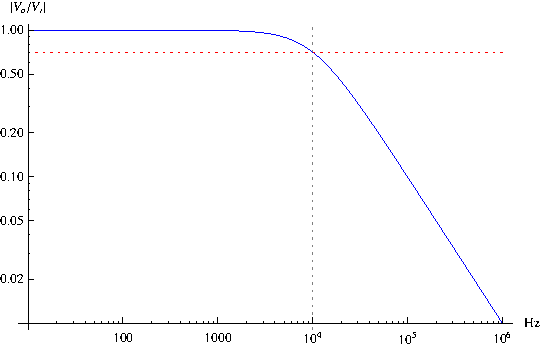
\includegraphics[scale=1.75]{Graphics/lpf_magnitude_plot}

%%% Phase plot source code (Mathematica) %%%
\begin{comment}
LogLinearPlot[
 {-ArcTan[1, (\[Omega]*2*Pi) R c] * 180/Pi,
   -45}
 , {\[Omega], 10, 10^6},
  PlotStyle -> {Blue, {Red, Dotted}},
 AxesLabel -> {Hz, "Degrees"},
 GridLines -> {{10^4}, None},
 GridLinesStyle -> Dotted,
 PlotRange -> Full,
 Ticks -> {Automatic, Union[{-45}, Range[0, -90, -10]]}]
\end{comment}
%%% End phase plot source code %%%

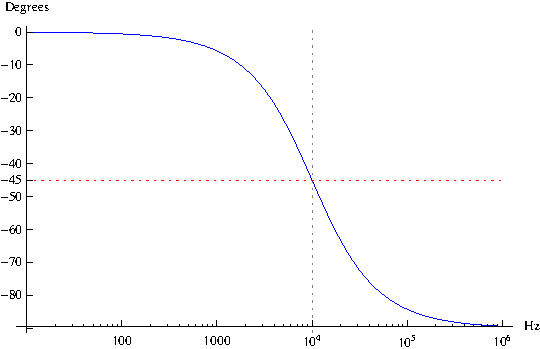
\includegraphics[scale=1.75]{Graphics/lpf_phase_plot}

The filter above has a \emph{break frequency} (also known as corner frequency, -3 dB point or $\displaystyle \frac{1}{\sqrt{2}}$ point) of 10 kHz, which means frequencies higher than 10 kHz will get attenuated. As you can see, however, the attenuation starts off lower than 10 kHz. The break frequency is the frequency where the magnitude drops to 3 dB below unity (1x the input), which equals $\displaystyle \frac{1}{\sqrt{2}}$ times unity, here shown by a pair of dotted lines. The break frequency is also where the phase shift of the signal is exactly -45 degrees (for this circuit).\\

There are 4 main types of filters: low-pass, high-pass, band-pass and band-stop. The names explain them quite well; low-pass filters let low frequencies through, but blocks higher ones, while high-pass is the exact opposite. Band-pass lets a \emph{band} of frequencies through, but blocks both lower and higher frequencies. Band-stop are opposite of band-pass; they let everything \emph{except} a band of frequencies through.

\subsection{Series RLC band-pass filter}

Since producing good-looking Bode plots for this document takes a while with my current process, I'll only make a few, by focusing on a RLC band-pass filter.

\begin{circuitikz}[scale=1.2]
\draw (0,0) node [ground] {} to [sV=$V_i$] (0,3)
					  to [L=$L$]     (3,3)
					  to [C=$C$]     (6,3)
					  to [R=$R$]	(6,0);
\draw (6,0) to [short, -o] (8,0);
\draw (6,3) to [short, -o] (8,3);
\draw (8,3) to [open, v=$V_o$] (8,0);
\draw (6,0) to (0,0);
\end{circuitikz}

First, let's think about how this filter works intuitively.\\
The inductor will let low frequencies through, but block high frequencies. Thus, at high frequencies, most of the circuit's voltage drop will be across the inductor, so the filter blocks them.\\
The capacitor will let the high frequencies pass with low impedance, but instead block low frequencies.\\
However, there is a band of frequencies somewhere in the middle that they both let through, so this is a \emph{band-pass} filter.\\

Since this is a series circuit, we can yet again use a simple voltage divider relation to write the transfer function $\displaystyle \frac{V_o}{V_i}$:

\[ \frac{V_o}{V_i} = \frac{R}{R + j\omega L + \frac{1}{j\omega C}} \]

Let's clean it up a bit by multiplying through by $j\omega C$.

\[ \frac{V_o}{V_i} = \frac{R}{R + j\omega L + \frac{1}{j\omega C}} \cdot \frac{j\omega C}{j\omega C} \]
\[ \frac{V_o}{V_i} = \frac{j\omega RC}{1 - \omega^2 LC + j\omega RC} \]

We can now calculate the magnitude and phase of the transfer function, and plot it.

\[ \left| \frac{V_o}{V_i} \right| = \frac{\omega RC}{\sqrt{(1 - \omega^2 LC)^2 + (\omega RC)^2}} \]
\[ \angle \frac{V_o}{V_i} = \frac{\pi}{2} - \arctan{(1 - \omega^2 LC, \omega RC)} \]

Here are the Bode plots for this circuit for $L = 1 \mu H$, $C = 1 \mu F$ and $R = 20 \Omega$:

%%% Mag. plot source %%%
\begin{comment}
LogLogPlot[{mag, 1/Sqrt[2]}, {\[Omega], 10, 10^9}, 
 PlotStyle -> {Blue, {Red, Dotted}}, 
 AxesLabel -> {Hz, 
   "|\!\(\*SubscriptBox[\(V\), \(o\)]\)/\!\(\*SubscriptBox[\(V\), \
\(i\)]\)|"}, 
 GridLines -> {{3.1910*10^6, 7937.95, 1/(2*Pi*Sqrt[L*c])}, None}, 
 GridLinesStyle -> Dotted]
\end{comment}
%%% End mag plot source %%%

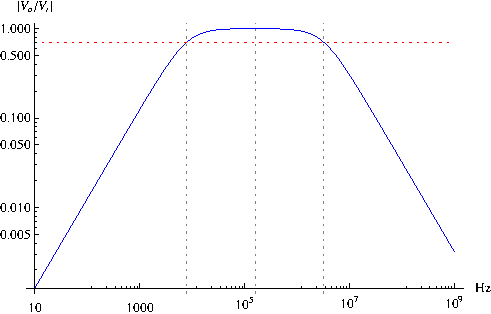
\includegraphics[scale=1.75]{Graphics/bpf_magnitude_plot}

The dotted red line is at $\displaystyle \frac{1}{\sqrt{2}}$. The dotted vertical lines are, from left to right, the low-end break frequency $f_1$, the resonant frequency $\displaystyle f_0 = \frac{1}{2\pi \sqrt{LC}}$ and the high-end break frequency $f_2$.\\
Note that the $f$ notation instead of $\omega$ indicates that the frequencies are in hertz, rather than rad/s.

%%% Phase plot source %%%
\begin{comment}

LogLinearPlot[{(\[Pi]/2 - 
     ArcTan[1 - (\[Omega]*2*Pi)^2 L c, (\[Omega]*2*
         Pi) R c])*(180/\[Pi]), 45, -45, 0}, {\[Omega], 10, 10^9}, 
 PlotStyle -> {Blue, {Red, Dotted}, {Red, Dotted}, {Red, Dotted}}, 
 AxesLabel -> {Hz, "Degrees"}, GridLinesStyle -> Dotted, 
 PlotRange -> Full, 
 Ticks -> {Automatic, Union[{-45, 45}, Range[90, -90, -10]]},
 GridLines -> {{3.1910*10^6, 7937.95, 1/(2*Pi*Sqrt[L*c])} , None}]
\end{comment}
%%% End phase plot source %%%

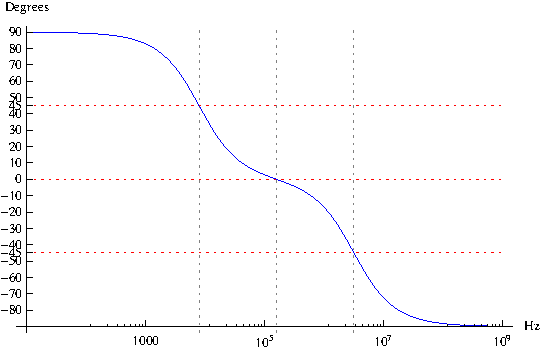
\includegraphics[scale=1.75]{Graphics/bpf_phase_plot}

The dotted red lines are at 45, 0 and -45 degrees. The dotted vertical lines are, from left to right, the low-end break frequency $f_1$, the resonant frequency $\displaystyle f_0 = \frac{1}{2\pi \sqrt{LC}}$ and the high-end break frequency $f_2$.\\

These plots show two break frequencies, at roughly 7.94 kHz and 3.19 MHz, respectively. (I have no idea where such a filter could be useful, however; the circuit values could've been better chosen for this example!)\\
The break frequencies can be found by setting the magnitude equation equal to $\displaystyle \frac{1}{\sqrt{2}}$ and solving for $\omega$ (keep in mind that $\omega$ is in rad/s; the plots are in hertz).\\

\newpage

\subsection{Q and ``peakiness''}
Something interesting happens if we observe the capacitor voltage of a high-Q RLC circuit near the resonant frequency.

\begin{circuitikz}[scale=1.2]
\draw (0,0) node [ground] {} to [sV=$V_i$] (0,3)
					  to [L=$L$]     (3,3)
					  to [C=$C$, v=$V_c$]     (6,3)
					  to [R=$R$]	(6,0);
\draw (6,0) to (0,0);
\end{circuitikz}
\\

%%%% Magnitude plot source code (Mathematica) %%%
\begin{comment}
Manipulate[
 LogLogPlot[{1/Sqrt[(1 - c L \[Omega]^2)^2 + (\[Omega] R c)^2], 
   1/Sqrt[2], 1/Sqrt[L*c] * L/R}, {\[Omega], 10, 10^6}, 
  PlotStyle -> {Blue, {Red, Dotted}, {Red, Dotted}}, 
  AxesLabel -> {Hz, 
    "|\!\(\*SubscriptBox[\(V\), \(o\)]\)/\!\(\*SubscriptBox[\(V\), \
\(i\)]\)|"}, GridLines -> {None, None}, GridLinesStyle -> Dotted, 
  PlotRange -> Full]
 , {R, 0.01, 1000}, {c, 10^-9, 10^-6}, {L, 10^-9, 10^-3}]

% Values used: R = 7.5, c = 4 * 10^-7, L = 0.75 * 10^-3 which causes Q ~ 5.7735
\end{comment}
%%% End magnitude plot source code %%%

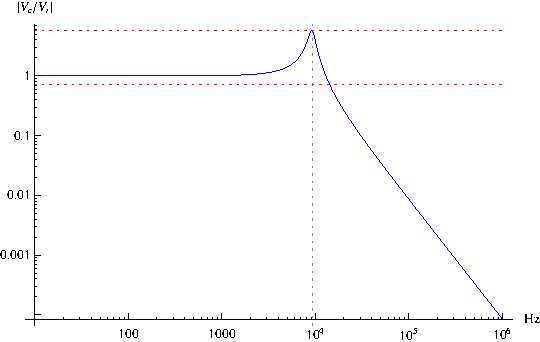
\includegraphics[scale=1.75]{Graphics/lpf_peakiness}

The above Bode plot shows the magnitude of the capacitor voltage/input voltage ratio for the values $R = 7.5 \Omega$, $L = 0.75$ mH, $c = 400$ nF, which causes $\displaystyle f_0 = \frac{1}{2\pi \sqrt{0.75\cdot10^{-3} \cdot 400 \cdot 10^{-9} }} \approx 9.19$ kHz and $\displaystyle Q = \frac{0.75 \cdot 10^{-3}}{7.5 \sqrt{0.75 \cdot 10^{-3} \cdot 400 \cdot 10^{-9}}} \approx 5.7735$.\\
The dotted red lines are at $\displaystyle \frac{1}{\sqrt{2}}$ and $Q$, while the dotted grey line is at $f_0 \approx 9.19$ kHz.\\

This phenomenon is actually not as strange as it may appear. Q is the ratio of stored energy in a circuit to the energy dissipated per cycle, so at high Q values, more energy is added by the source than is dissipated by the resistor, so the voltage builds up over time, to be greater than the input amplitude (specifically $Q$ times greater).

Let's derive this mathematically. Again, this was for the voltage over the capacitor, so we need to calculate the magnitude of that. Yet again we used a voltage divider relation:

\[ \frac{V_c}{V_i} = \frac{\frac{1}{sC}}{\frac{1}{sC} + sL + R} \]

Multiply across by $sC$ to clean up:

\[ \frac{V_c}{V_i} = \frac{1}{1 + s^2LC + sRC} \]

Let's divide through by $LC$, too:

\[ \frac{V_c}{V_i} = \frac{\frac{1}{LC}}{s^2 + \frac{R}{L} s + \frac{1}{LC}} \]

There's the characteristic equation again. We know (from memory, but also from comparing the above to $s^2 + 2\alpha s + {\omega_0}^2$) that $\displaystyle \frac{1}{LC} = {\omega_0}^2$, and the same goes for $\displaystyle 2 \alpha = \frac{R}{L}$.

\[ \frac{V_c}{V_i} = \frac{{\omega_0}^2}{s^2 + 2 \alpha s + {\omega_0}^2} \]

$s = j\omega$; however, let's evaluate the above expression at the resonant frequency, i.e. $\omega = \omega_0$, so we make the substitution for $s = j\omega_0$:

\[ \frac{V_c}{V_i} = \frac{{\omega_0}^2}{(j\omega_0)^2 + 2 \alpha j\omega_0 + {\omega_0}^2} \]

$j^2$ is $-1$, so:

\[ \frac{V_c}{V_i} = \frac{{\omega_0}^2}{-{\omega_0}^2 + 2 \alpha j\omega_0 + {\omega_0}^2} \]

Each term has an $\omega_0$, so we can cancel them out. 

\[ \frac{V_c}{V_i} = \frac{{\omega_0}}{-{\omega_0} + j 2 \alpha + {\omega_0}} \]


Also, note that we have $-\omega_0 +\omega_0$ remaining, so we remove those as well:

\[ \frac{V_c}{V_i} = \frac{{\omega_0}}{j 2 \alpha} \]

We then take the magnitude of this expression, that (remember what we're doing!) shows the ratio of the capacitor voltage to the input, at the circuit's resonant frequency. The only thing that happens is that $j$ disappears, as its magnitude is $1$:

\[ \left| \frac{V_c}{V_i} \right| = \frac{\omega_0}{2\alpha} = Q \]

Yup! It turns out that the Bode plot is correct: the magnitude of the capacitor voltage at resonance is exactly $Q$ times greater than $V_i$!


\subsection{Selectivity and bandwidth}
The selectivity of a filter is given by 
\[ \frac{\omega_0}{\Delta \omega} \]
where $\Delta \omega$ is the \emph{bandwidth} of the filter:

\[ \Delta \omega = \omega_2 - \omega_1 \]
where $\omega_1$ and $\omega_2$ are the $\displaystyle \frac{1}{\sqrt{2}}$ points of the filter (see above).\\
For the filter above:

\[ \omega_0 = \frac{1}{2\pi \sqrt{LC}} = 159.2 \text{ kHz} \]
\[ \omega_1 = 7.938 \text{ kHz} \]
\[ \omega_2 = 3.191 \text { MHz} \]
\[ \Delta \omega = \omega_2 - \omega_1 = 3.183 \text{ MHz} \]
\[ \frac{\omega_0}{\Delta \omega} \approx 0.05 \]

Let's try to find $\displaystyle \frac{\omega_0}{\Delta \omega}$ in terms of circuit parameters, e.g. R, C, L and so on.\\
To begin with, we set the magnitude equation equal to $\displaystyle \frac{1}{\sqrt{2}}$. We solve it, and take the two positive solutions, $\omega_2$ and $\omega_1$, and subtract them. The result is the bandwidth, $\Delta \omega$.\\
Of course, we already know that for a series RLC circuit, $\displaystyle \omega_0 = \frac{1}{\sqrt{LC}}$.

\[ \frac{\omega RC}{\sqrt{(1 - \omega^2 LC)^2 + (\omega RC)^2}} = \frac{1}{\sqrt{2}} \]

The solutions $\omega_1$ and $\omega_2$ to the above are quite messy, but when subtracted, the end result is very simple:

\[ \Delta \omega = \omega_2 - \omega_1 = \frac{R}{L} \]

Nice! Let's confirm that the previous result for $\Delta \omega$ matches this one:

\[ \Delta \omega = \omega_2 - \omega_1 = 3.191 \text{ MHz} - 7.938 \text{ kHz} = \frac{20 \Omega}{2\pi \cdot 1 \mu H} \]
Note that we need to additionally divide by $2 \pi$ to convert from rad/s to hertz. And indeed, the above is true, excepting for rounding errors.\\
However, there is an additional thing to note here. Remember that $\displaystyle 2 \alpha = \frac{R}{L}$ for a series RLC circuit! Thus the bandwidth $\Delta \omega$ is equal to $2 \alpha$.\\
Further, remember the definition of Q for the series RLC circuit:

\[ Q = \frac{\omega_0}{2\alpha} \]

We've just shown that $\Delta \omega = 2 \alpha$, so the selectivity of a circuit is given by Q!

Or, in circuit parameters:

\[ Q = \frac{L}{R \sqrt{LC}} \]


\subsection{Designing filters}
Instead of simply analyzing existing circuits, let's design a band-stop filter. Let's say we want it to stop frequencies in the range 1 - 10 kHz. In other words, we want the break frequencies to be at 1 and 10 kHz, respectively, which gives a bandwidth $\Delta \omega$ of 9 kHz.\\

Again, let's approach this intuitively. Clearly, a resistor combined with either a capacitor or inductor won't cut it, since such a circuit can only block either low or high frequencies (as the (ideal) resistor blocks all frequencies equally), not any sort of a combination. Thus we need either a RLC circuit, or some circuit consisting of multiple capacitors/multiple inductors. One solution would indeed be an RLC circuit, where we take the output over the LC pair rather than over the resistor as we did in the band-\emph{pass} filter above:

\begin{circuitikz}[scale=1.2]
\draw (0,0) node [ground] {} to [sV=$V_i$] (0,3)
					  to [R=$R$]     (3,3)
					  to [L=$L$]     (3,1.5)
					  to [C=$C$]	(3,0);
\draw (3,0) to [short, -o] (5,0);
\draw (3,3) to [short, -o] (5,3);
\draw (5,3) to [open, v=$V_o$] (5,0);
\draw (3,0) to (0,0);
\end{circuitikz}

\ \\
In this circuit, the LC voltage will be high either when the frequency is low (the capacitor drops a lot of voltage) or high (the inductor drops a lot of voltage), but low at some frequency band in between. Great!\\
Let's figure out the part values we want, and all that. First, we need to figure out the circuit's transfer function:

\[ \frac{V_o}{V_i} = \frac{sL + \frac{1}{sC}}{R + sL + \frac{1}{sC}} \]
where $s = j\omega$. We multiply through by $sC$ to get rid of the nested fractions:

\[ \frac{V_o}{V_i} = \frac{s^2LC + 1}{1 + sRC + s^2LC} \]

Hmm, let's clean up that $s^2$ term in the denominator by dividing by LC throughout.

\[ \frac{V_o}{V_i} = \frac{s^2 + \frac{1}{LC}}{\frac{1}{LC} + \frac{R}{L} s + s^2} \]

There's the characteristic equation for this circuit (in the denominator). If we match it up with the canonical form $s^2 + 2\alpha s + {\omega_0}^2$, we find that

\[ 2\alpha = \frac{R}{L} \]
\[ \alpha = \frac{R}{2L} \]
\[ {\omega_0}^2 = \frac{1}{LC} \]
\[ \omega_0 = \frac{1}{\sqrt{LC}} \]

This isn't really news, since we knew the values of $\alpha$ and $\omega_0$ for the series RLC circuit already, but it's nice to know we can find them easily. Let's find out the values of $Q$ and $\Delta \omega$, the bandwidth:

\[ Q = \frac{w_0}{2\alpha} = \frac{ \frac{1}{\sqrt{LC}} }{ \frac{R}{L} } = \frac{L}{R\sqrt{LC}} \]
\[ \Delta\omega = 2 \alpha = \frac{R}{L} \]

Then, let's calculate the magnitude and phase equations. Let's go back to the form we had before we divided through by LC, since it looks a bit cleaner. Let's then make the substitution for $s = j\omega$, and see what happens:

\[ \frac{V_o}{V_i} = \frac{s^2LC + 1}{1 + sRC + s^2LC} \]
\[ \frac{V_o}{V_i} = \frac{(j\omega)^2 LC + 1}{1 + j\omega RC + (j\omega )^2 LC} \]
\[ \frac{V_o}{V_i} = \frac{1 - \omega^2 LC}{1 - \omega^2 LC + j\omega RC} \]

I simply made the substitution, then sorted the terms to be real followed by imaginary, to make things easier in the next step. We're now ready to calculate the magnitude and phase $\displaystyle \left| \frac{V_o}{V_i} \right|$ and $\displaystyle \angle \frac{V_o}{V_i}$:

\[ \displaystyle \left| \frac{V_o}{V_i} \right| = \frac{|1 - \omega^2 L C|}{\sqrt{(1 - \omega^2 LC)^2 + (\omega RC)^2}} \]
\[ \displaystyle \angle \frac{V_o}{V_i} = 0 - \arctan{(1 - \omega^2 LC, \omega RC)} \]

Now we're getting somewhere. Let's see, what were our requirements? We wanted the filter to block out 1 - 10 kHz (i.e. we want a 9 kHz bandwidth for the blocked frequencies). Let's set the break frequencies at those two points.\\
Let's choose $R = 10 \Omega$, to reduce the variable count and make the rest more easily doable.

We need to find the break frequencies in terms of the circuit variables. To do so, we set the magnitude equation equal to $\displaystyle \frac{1}{\sqrt{2}}$ and solve:

\[ \frac{|1 - \omega^2 L C|}{\sqrt{(1 - \omega^2 LC)^2 + (\omega RC)^2}} = \frac{1}{\sqrt{2}} \]

I used Mathematica for this, and got four roots; two of those will give us negative numbers for the frequencies, so they were discarded. The two solutions that remained were, after simplification:

\[ \omega_1 = \frac{2}{RC + \sqrt{4LC + (RC)^2}} \]
\[ \omega_2 = \frac{R + \sqrt{4\frac{L}{C} + R^2}}{2L} \]

Let's set up a system of equations, where $\omega_1$ is equal to the low break frequency, and $\omega_2$ is equal to the higher one:

\[ \frac{2}{RC + \sqrt{4LC + (RC)^2}} = 2\pi \cdot 10^3 \]
\[ \frac{R + \sqrt{4\frac{L}{C} + R^2}}{2L} = 2\pi \cdot 10^3 \]

If we solve these simultaneous equations, the answers given are
\[ L = \frac{R}{1800\pi} \]
\[ C = \frac{9}{200000\pi R} \]

So, for $R = 10 \Omega$, the values are roughly $L = 0.1768$ mH and $C = 14.324\mu$F.\\

Here are the Bode plots for the resulting filter:

\begin{comment}
%%% BSF magnitude plot source code
LogLogPlot[{Abs[1 - (\[Omega]*2*Pi)^2 L c]/
   Sqrt[(1 - (\[Omega]*2*Pi)^2 L c)^2 + ((\[Omega]*2*Pi) R c)^2], 
  1/Sqrt[2]}, {\[Omega], 10, 10^6}, 
 PlotStyle -> {Blue, {Red, Dotted}}, 
 AxesLabel -> {Hz, 
   "|\!\(\*SubscriptBox[\(V\), \(o\)]\)/\!\(\*SubscriptBox[\(V\), \
\(i\)]\)|"}, GridLines -> {{10^3, 10^4}, None}, 
 GridLinesStyle -> Dotted, PlotRange -> {{10, 10^6}, {0.01, 1}}]
%%% End source
\end{comment}

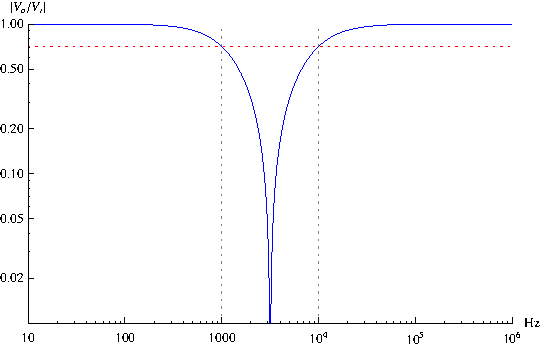
\includegraphics[scale=1.4]{Graphics/bsf_magnitude_plot}

As with the previous plots, the dotted red line is at $\displaystyle \frac{1}{\sqrt{2}}$ and the dotted grey lines are at the break frequencies, i.e. 1 and 10 kHz.\\
The $Q$ of this filter is approximately $0.3514$.

\begin{comment}
%%% BSF phase plot source code
f[x_] = If[x < -\[Pi]/2, x + \[Pi], x]

LogLinearPlot[{f[-ArcTan[
      1 - (\[Omega]*2*Pi)^2 L c, (\[Omega]*2*Pi) R c]]*180/Pi, -45, 
  45}, {\[Omega], 10, 10^6}, 
 PlotStyle -> {Blue, {Red, Dotted}, {Red, Dotted}}, 
 AxesLabel -> {Hz, "Degrees"}, GridLines -> {{10^3, 10^4}, None}, 
 GridLinesStyle -> Dotted, PlotRange -> Full, 
 Ticks -> {Automatic, Union[{-45, 45}, Range[90, -90, -10]]}]
%%% End source
\end{comment}

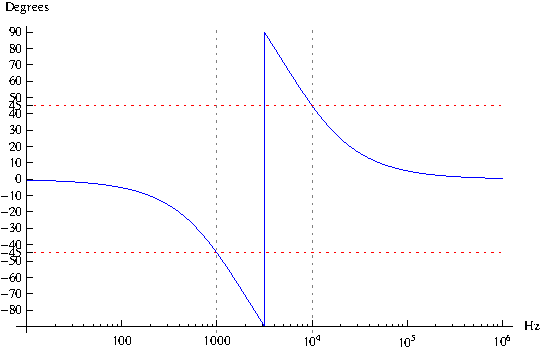
\includegraphics[scale=1.4]{Graphics/bsf_phase_plot}

Note the discontinuity in the plot, due to us restricting the valid range of phase values between +90 and -90 degrees.\\
Without the discontinuity, the phase plot looks like this:

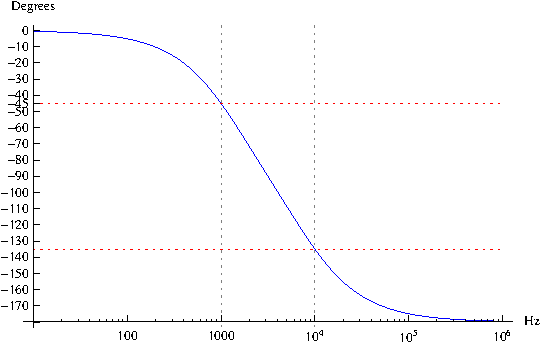
\includegraphics[scale=1.4]{Graphics/bsf_phase_plot_no_disc}

It looks like our filter works! However, there are some caveats here. For one, in actual circuits, it's hard to find $\approx 14 \mu$F capacitors that are suitable for filters, due to nonlinearities in electrolytic capacitors. (Most capacitors with values higher than the low-microfarad range are electrolytics; especially once you get to far higher capacitance values.)\\
In addition, they are usually polarized, and as such cannot tolerate negative voltages.\\
Also, the current through this filter will be very high if the signal source has a low impedance.\\
All in all, however, it pretty much works - not bad for a first-ever try in filter design, especially  considering that low-pass/high-pass filters with only two components are quite a bit easier.

\newpage

\section{Summary of SSS, impedance and filters}
This chapter dealt with the steady state workings of circuits with sinusoidal input. We learned that, by representing this as an exponential input, we can turn the differential equations governing these circuits into simple algebraic relations: \emph{the impedance model}. In doing so, we not only got access to easy tools for frequency domain analysis of circuits, but also a few that also help us in the time domain, such as the equation for converting a complex amplitude, used in the impedance model, to a time domain representation of the circuit:

\[ v_X(t) = |V_x| \cos{(\omega t + \angle V_x)} \]

The impedances (denoted by $Z$) for the three common passive circuit elements\footnote{There are four such basic elements; the fourth is the memristor, which as of this writing is still under development, with commercial release slated for 2013.} are:

\[ \text{Resistor: } Z_R = R \]
\[ \text{Capacitor: } Z_C = \frac{1}{j\omega C} \]
\[ \text{Inductor: } Z_L = j\omega L \]

The most important parameters for filters are:\\
(Where specific circuit parameters are used, they are for the series RLC circuit. The parameters themselves ($\alpha$, $\Delta \omega$ etc.) apply to all circuits, however.)

\[ \text{Resonant angular frequency: } \omega_0 = \frac{1}{\sqrt{LC}} \text{ rad/s} \]
\[ \text{Resonant frequency: } f_0 = \frac{1}{2\pi \sqrt{LC}} \text { Hz} \]
\[ \text{Damping factor: } \alpha = \frac{R}{2 L} \text{ rad/s} \]
\[ \text{Bandwidth: } \Delta \omega = \omega_2 - \omega_1 = 2 \alpha = \frac{R}{L} \text { rad/s} \]
\[ Q = \frac{\omega_0}{2 \alpha} \text{ (dimensionless)} \]

Remember that $Q$ can be thought of as multiple things. For a frequency-domain analysis, it is indicative of the how selective the filter is. High Q means high selectivity.\\
For time-domain analyses, Q indicates how long an underdamped system will ring; also, systems with $\displaystyle Q < \frac{1}{2}$ are overdamped and will not ring at all.


%%%%%%%%%%%%%%%%%%%%%
%%% Miscellaneous %%%
%%%%%%%%%%%%%%%%%%%%%

\chapter{Miscellaneous}
\section{Impulses and steps}

\subsection{A note}
For a linear circuit - one with resistors, capacitors and inductors \emph{ONLY} - no sources allowed - an interesting relation between input and output exists. If y(t) is the output for the input x(t), the output for the derivative of x(t) will be the derivative of y(t). The same goes for integration. That is,

\[ x(t) \to y(t) \]
\[ x'(t) \to y'(t) \]
\[ \int x(t) dt \to \int y(t) dt \]

The usefulness for this will soon be clear. In a short preview, we can calculate the behaviour of such a circuit to for example an impulse, and then integrate the response we got; the integrated answer will then be the circuit response to a \emph{step}, as a step is the result of integrating an impulse.

\subsection{Impulses}
Impulses are (theoretical) bursts of an infinite voltage/current over an infinitesimally small time. The Dirac Delta function, $\delta(t)$, is used to describe them. The delta function is defined as\footnote{Perhaps not rigorously, but good enough for our purposes.}

\[ \delta(x) = \begin{cases}
   +\infty & x = 0 \\
   0       & x \neq 0
   \end{cases}
\]
In other words, it is zero everywhere except at $x = 0$, where it's infinite. There is an additional identity it is constrained to, however:

\[ \int_{-\infty}^{\infty} \delta(x) dx = 1 \]
In other words, the area under the curve is exactly 1. Mathematically, the delta function is not a proper function, but can be defined as a distribution.

In a parallel, current source-driven RC circuit, a current impulse at $t = 0$ delivers 100\% of its charge to the capacitor, and essentially creates an initial condition for $t = 0^{+}$. Assuming the capacitor has no state, the capacitor voltage after the impulse will be 

\[ v_C(0^{+}) = \frac{Q}{C} \]

where Q is the area of the impulse, i.e. the current source output is given by

\[ Q \delta(t) \], so Q is in coulombs, the SI unit for electric charge. The unit is such that

\[ \frac{1\text{ coulomb}}{1\text{ farad}} = 1\text{ volt} \]

In such a circuit, the capacitor voltage (and thus the entire circuit's voltage, as there is only 1 node besides ground) for $t > 0^{+}$ will be given by

\[ v_C(t) = \frac{Q}{C} e^{-\frac{t}{RC}} \]

The dual of this circuit is the series RL circuit, with a voltage source, a resistance and an inductance. In this case, we have a voltage impulse, that delivers a flux linkage $\Lambda$ to the inductor. As above, this will essentially create an initial condition, this time for the inductor current. Assuming the inductor has no state, the current through it will be:

\[ i_L(0^{+}) = \frac{\Lambda}{L} \]

where $\Lambda$ is the area of the impulse, i.e. the voltage source output is given by

\[ \Lambda \delta(t) \], so $\Lambda$ is in webers, the SI unit for magnetic flux. The unit is such that
\[ \frac{1\text{ weber}}{1\text{ henry}} = 1\text{ ampere} \]

Again, an in the previous case (the circuits are duals, after all), the inductor current for $t > 0^{+}$ is given by

\[ i_L(t) = \frac{\Lambda}{L} e^{-\frac{R t}{L}} \] 

\subsection{Steps}
Steps are the result of integrating an impulse. Steps are likely more intuitive than impulses. The unit step function (or the \emph{Heaviside step function}) has the definition

\[ u(t) = 
  \begin{cases}
   0  & t < 0 \\
   1  & t \ge 0
  \end{cases}
\]
In words, it ``turns on'' at $t = 0$, and so is a useful model for things such as a voltage source turning on at $t = 0$. Such a source could be written as

\[ V_I u(t) \]
where $V_I$ is the voltage of the source when turned on.\\

As noted in the introduction section, a step is the result of integrating an impulse. Thus, we can calculate the circuit response to a step by calculating the response to an impulse, and then integrate the answer.\\
In a similar manner, we can calculate the response to a step, and differentiate the answer to find the response to an impulse.

\subsection{Shifts}
The above functions can be shifted to start at times other than $t = 0$ by shifting them.\\
For example, while the unit step function $u(t)$ ``turns on'' at $t = 0$, we can make it turn on at time $t = 5$ by shifting it, like so: $u(t - 5)$\\
The above function will have $t - 5$ be negative until $t = 5$ where it becomes positive, and the unit step function changes its output from 0 to 1.\\
The exact same principle applies to the unit impulse function $\delta(t)$.

In general, for the change to happen at time $t = T$, use $u(t - T)$ or $\delta(t - T)$.

\end{document}